\appendix
\section{Φυσικό σχέδιο}\label{appendix:layout}

\begin{figure}[h!]
	\centering
	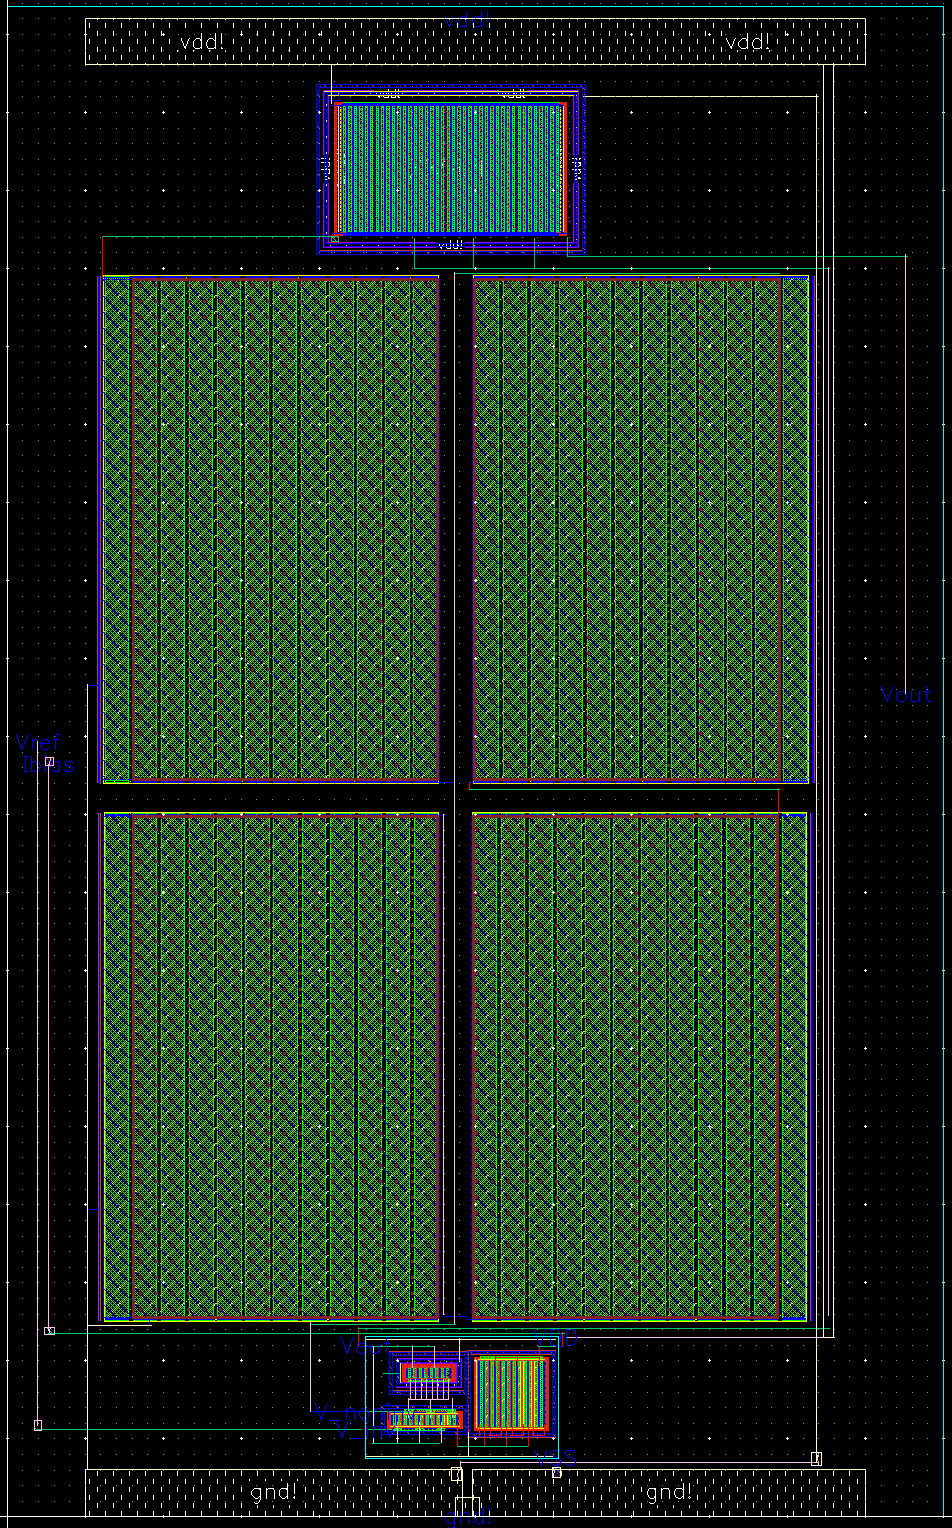
\includegraphics[width=0.92\linewidth]{assets/virtuoso/layout/ldo_layout_blackbg.png}
	\caption{Φυσικό σχέδιο του ρυθμιστή LDO.}
	\label{fig:error_amplifier:ldo:layout_black}
\end{figure}

\begin{figure}[p]
	\centering
	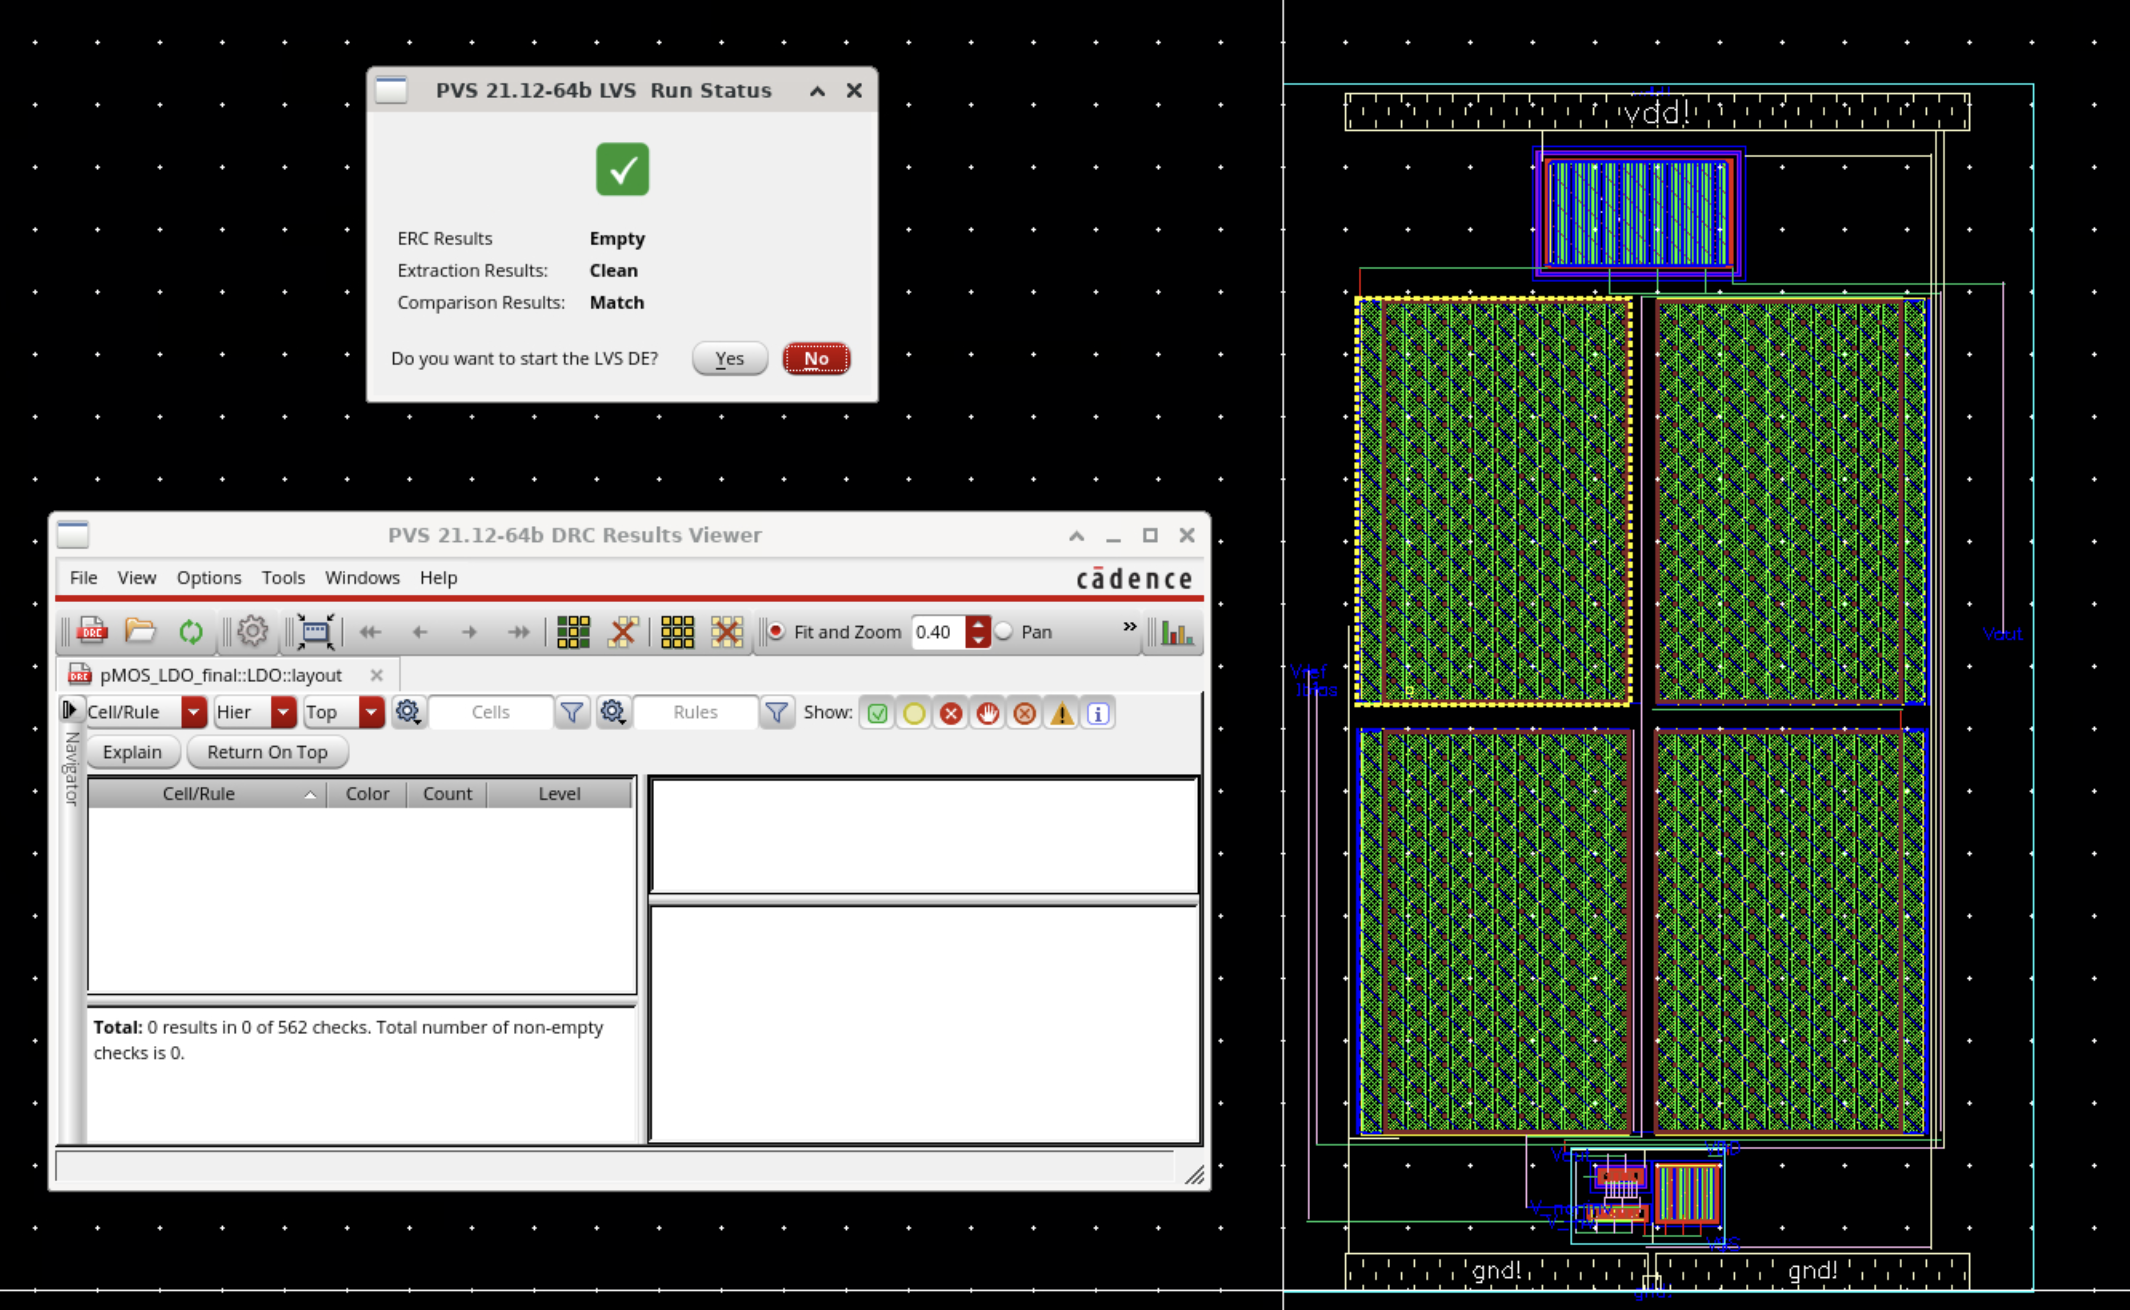
\includegraphics[width=\linewidth]{assets/virtuoso/layout/LDO_DRC_LVS.png}
	\caption{Στιγμιότυπο καθαρού ελέγχου DRC και επιτυχούς LVS ελέγχου για το φυσικό σχέδιο του LDO.}
	\label{fig:error_amplifier:ldo:layout_DRC_LVS}
\end{figure}
\clearpage

\begin{sidewaysfigure}[h!]
	\centering
	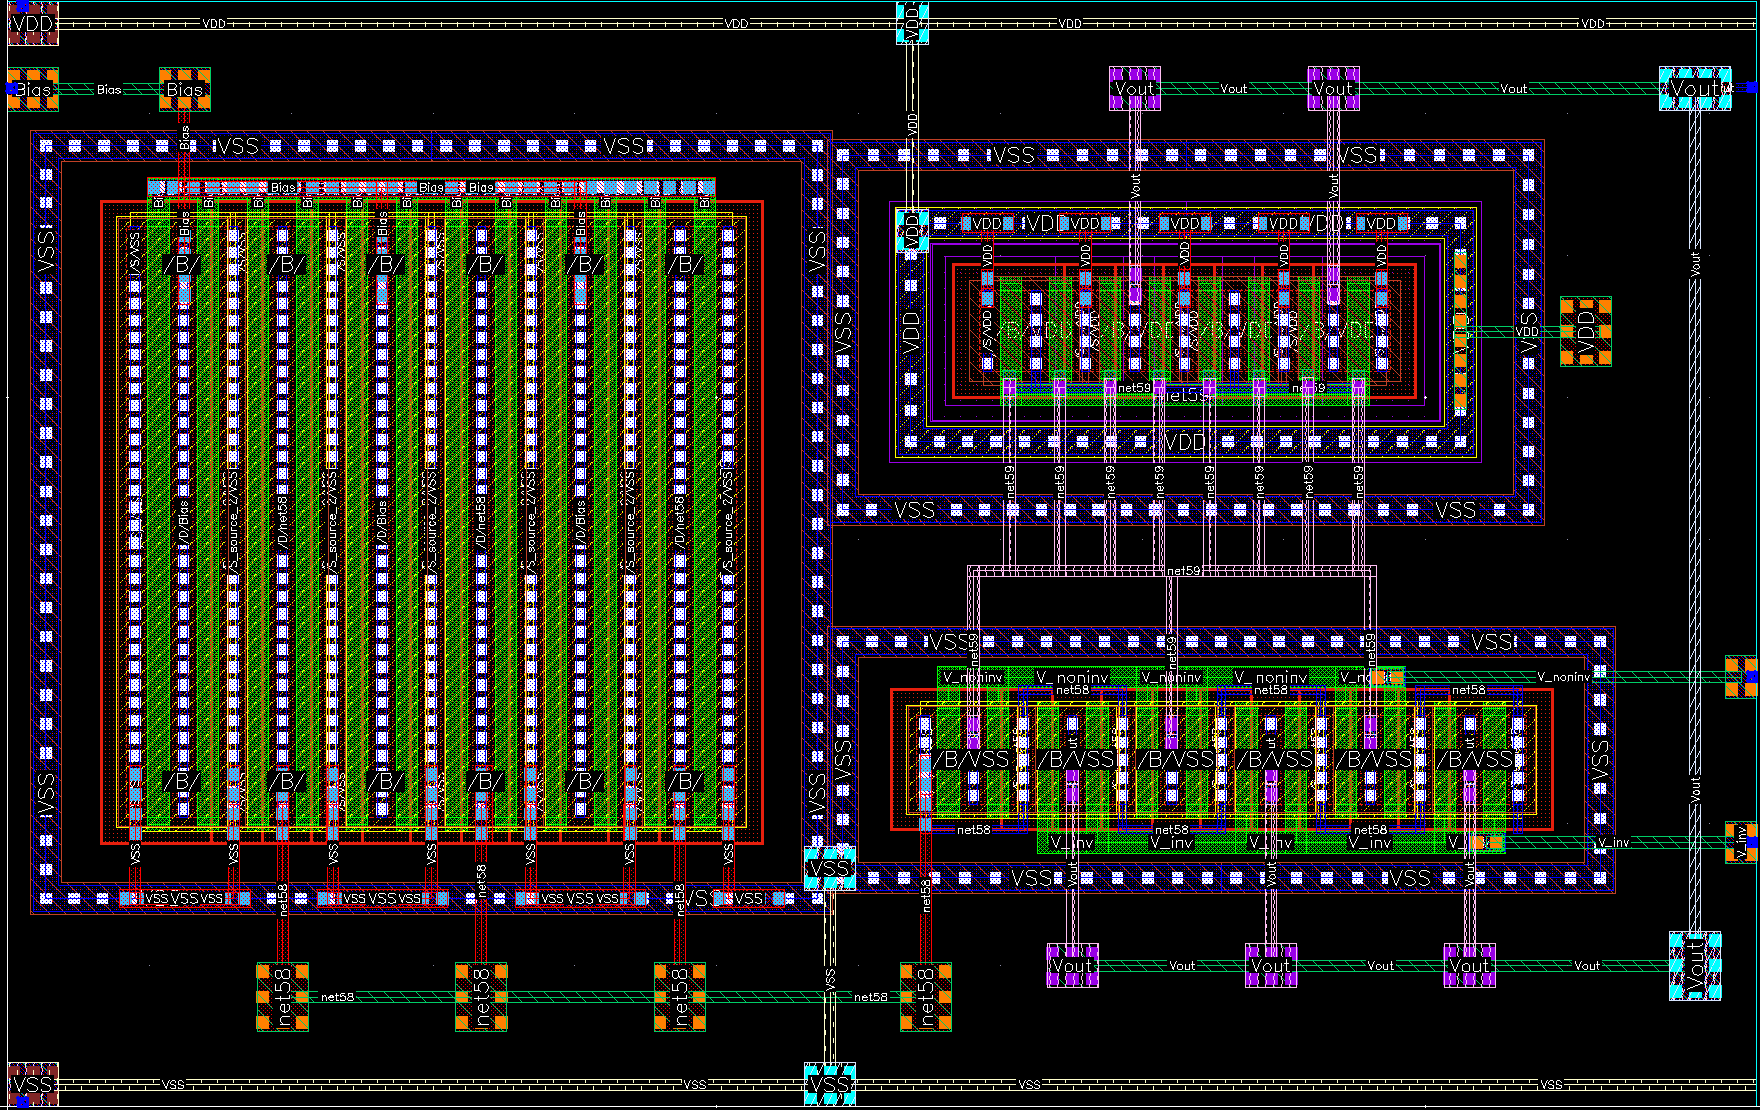
\includegraphics[width=0.9\linewidth]{assets/virtuoso/layout/error_amplifier_layout_blackbg.png}
	\caption{Φυσικό σχέδιο του ενισχυτή σφάλματος. Αριστερά: $\symup{N}_{5x}$-$\symup{N}_{6x}$. Δεξιά πάνω: $\symup{P}_{3x}$-$\symup{P}_{4x}$. Δεξιά κάτω: $\symup{N}_{1x}$-$\symup{N}_{2x}$.}
	\label{fig:error_amplifier:layout_black}
\end{sidewaysfigure}

\begin{figure}[p]
	\centering
	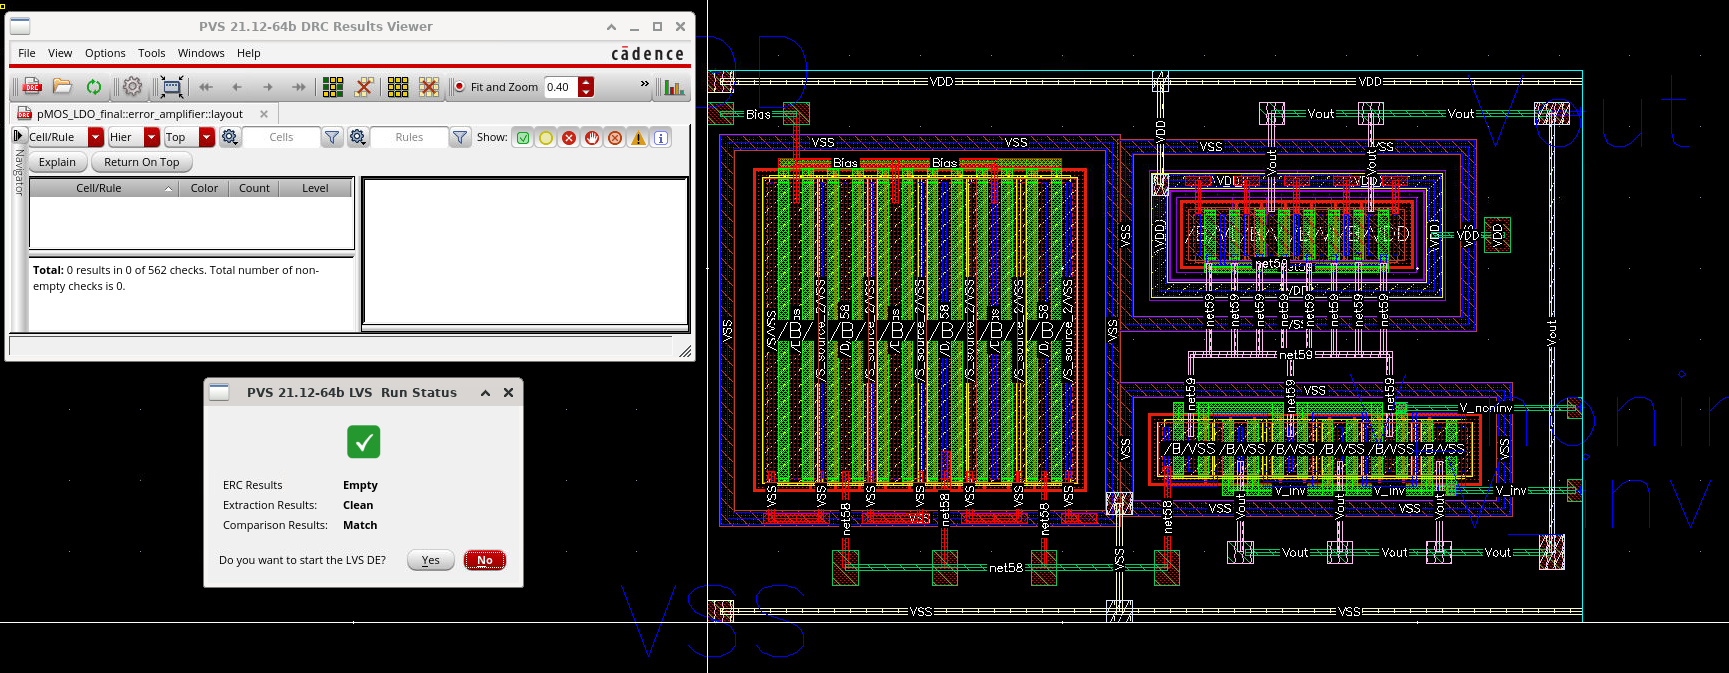
\includegraphics[width=\linewidth]{assets/virtuoso/layout/Error_amplifier_layout_checks.png}
	\caption{Στιγμιότυπο καθαρού ελέγχου DRC και επιτυχούς LVS ελέγχου για το φυσικό σχέδιο του ενισχυτή.}
	\label{fig:error_amplifier:layout_DRC_LVS}
\end{figure}
\clearpage